\chapter{手法の検討}
\label{consideration}

\section{概要}
第\ref{issue:siit-dc_problems}項で述べたように,現状のSIIT-DC及びEAMTの仕様はEAMTの一貫性を担保する手法の検討がなされておらず,それに起因した障害時の適切なフェイルオーバーの実行やIPv4サービスの増減時の変更追従に関しての課題がある.
NPO日本ネットワークセキュリティ協会(JNSA)らの調査によればITシステムの障害の原因の約半数は人為ミスに分類されるものにあり\cite{human_error},サービスの安定的な稼働を実現するためには単調な繰り返し動作を含む運用をシステムによって減らす必要がある.

本研究ではSIIT-DCにおけるダイナミックEAMT\footnote{BR群のEAMTをシステムにより動的に制御する機構}の実現を目指す.本章では考えられる手法を大別した上でその特徴と利点及び欠点を挙げ,最も適した手法を検討する.


\section{求められる要件}
\label{consideration:points}

第\ref{related:abstract:requirements}で述べたIPv4サービス提供手法の機能要件と,第\ref{issue:siit-dc_problems}項で挙げたSIIT-DCの現状の課題を総合し,EAMTを動的に制御する手法に求められる要件を下記のように定義した.

\subsubsection{BR間のEAMTの一貫性}
第\ref{issue:siit-dc_problems}項で述べたように,障害時の適切なフェイルオーバーを実現するためには,各BRのEAMTの一貫性が保証される必要がある.

\subsubsection{変更追従性}
近年のIDCでは多数の物理サーバーを統合的に管理するプライベートクラウド環境やコンテナオーケストレーション環境\footnote{Container Orchestration.コンテナ型仮想化統合管理環境}が普及しており,アプリケーション・サービスの追加及び削除が頻繁に行われている.サービスの障害時に適切にそれを検知し,適切に冗長系に移行するははSLB\footnote{Servver Load Balancer}を中心として広く利用されている.SIIT-DCのIPv4サービス提供の場でも,サービスの状態の変動にリニアに対応しフェイルオーバーできるような働きが求められる.

\subsubsection{スケーラビリティ}
第\ref{related:abstract:requirements}で述べたようにIPv6シングルスタックネットワークにおけるIPv4サービスの提供では水平スケールが容易に行える仕組みを備える必要がある.
IPv4サービスを行うサーバーの増設や,対外接続点が増えた場合のBRの拡大に十分に適用するスケーラビリティを有することが望ましい.

次項ではスケーラビリティの評価のために,制御に必要な通信コネクション数による比較を行う.以後BRの数を$M$,IPv4サービスを提供するサーバーの数を$N$とし,総通信コネクション数を$C$として表現する.


%
%\subsection{冗長性}
%EAMTを制御するために用いられる管理台帳となるデータは高可用性を有した形で保持する必要がある.EAMTを分散管理
%EAMTを制御するために用いられる管理台帳となるデータを保持するノードがいる場合,単一障害点になることを防ぐために高可用性クラスター\cite{gadir2005high}を構成できるアーキテクチャである必要がある.

\subsection{デプロイメントの容易さ}
第\ref{issue:siit-dc:network}で述べたように,SIIT-DCの最も特筆すべきメリットの一つにデプロイメントの容易さが挙げられる.
これを損なうこと無くダイナミックEAMTが導入されることが望ましい.


\section{アプローチの分類と比較}
本説ではダイナミックEAMTを実現するアプローチとして,二系統のアプローチを考案する.それぞれのアプローチで考えられる実装と実際の構成,及び第\ref{consideration:points}節で述べた各要件への適合を定性的に評価する.



\subsection{中央管理型アプローチ}
\label{consideration:approach:centerized}

\begin{figure}[h]
    \begin{center}
      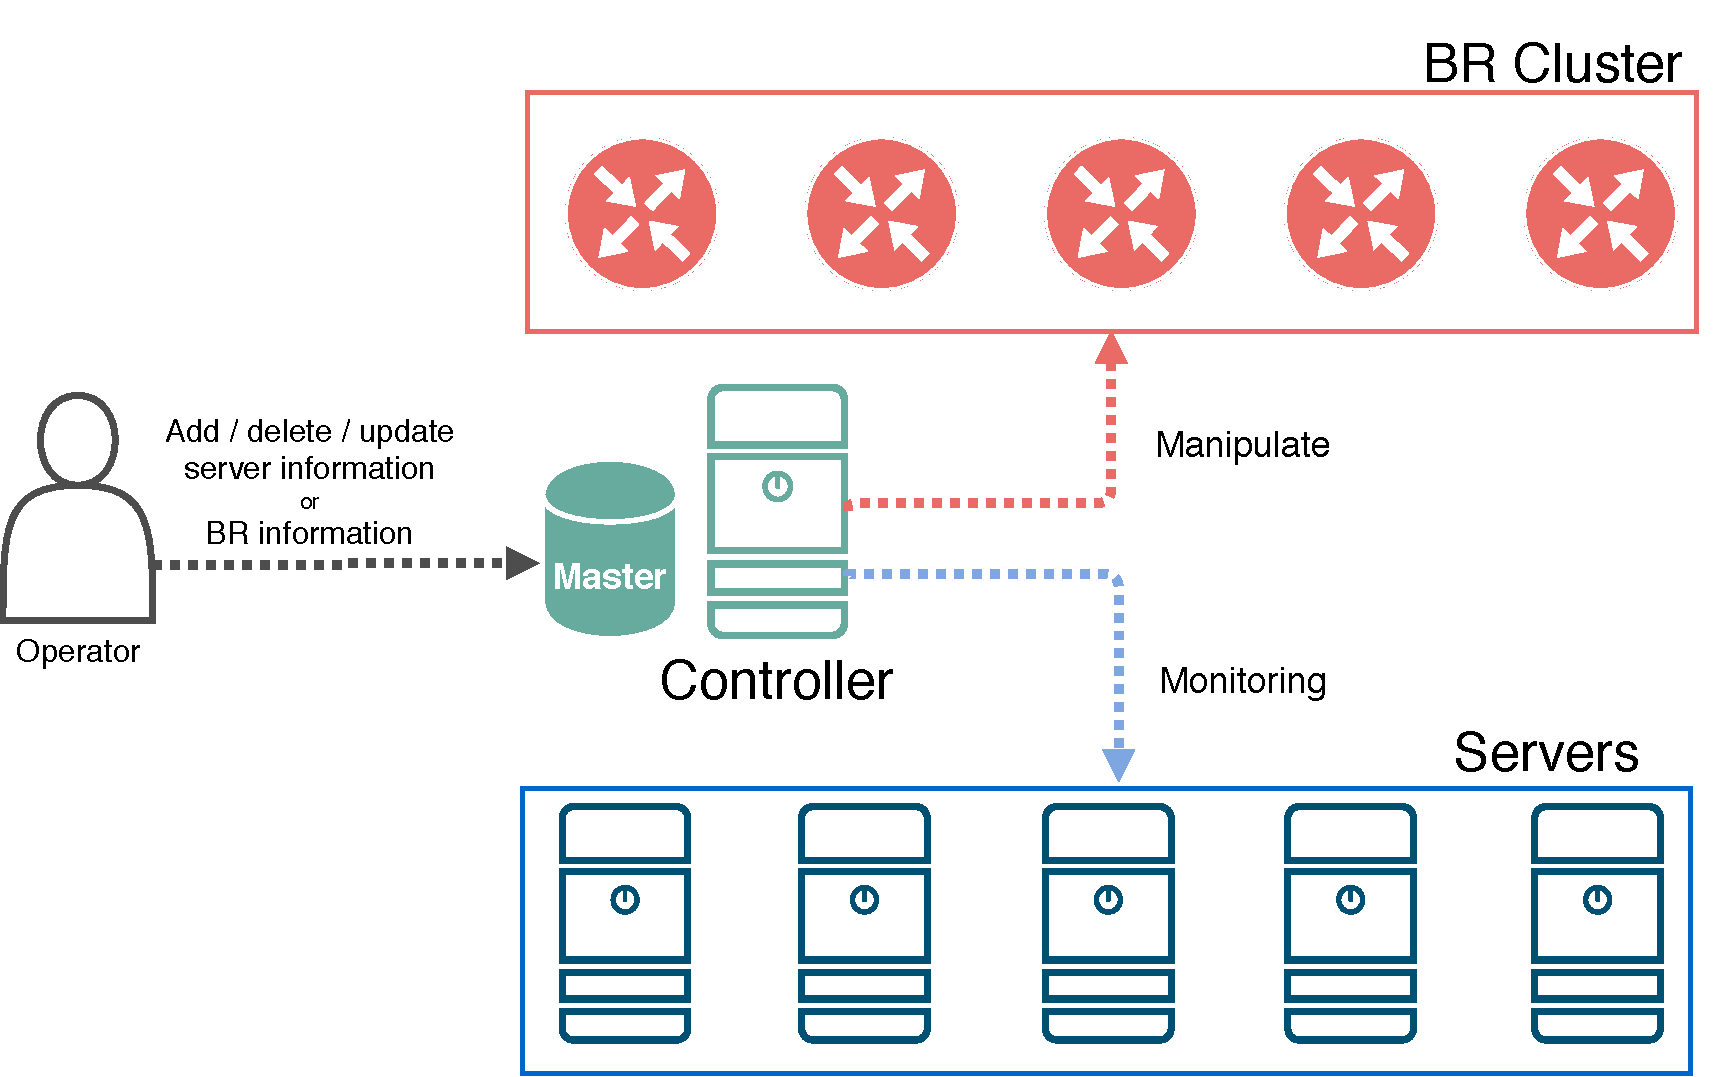
\includegraphics[width=12cm,pagebox=cropbox,clip]{img/approach_centerized_model.pdf}
    \end{center}
    \caption{中央管理型アプローチによるダイナミックEAMT}
    \label{fig:approach_centerized_model}
\end{figure}

中央管理型アプローチとは,複数のBRのEAMTを統合的に管理する「コントローラー」をIDCネットワーク上に配置し,各BRがネットワークを介してこれを参照する機構である.
図\ref{fig:approach_centerized_model}に中央管理型アプローチによってダイナミックEAMTを実現したSIIT-DCの各コンポーネントの関係図を表す.

中央管理型アプローチではコントローラーが各BRに投入するEAMが記録された「マスターテーブル」を保持し,それを元に各BRのデータプレーンにルールを書き込む手法を取る.マスターテーブルに記載されるEAMはオペレーターがネットワークの構成変更に合わせて追加・削除・更新を行い,それぞれのIPv4サービスを提供するサーバー群に対してはコントローラからプル型\footnote{pull-based monitoring. コントローラから各サーバーに能動的に情報を取得する}の外部監視\footnote{External monitoring}によりサーバーの状態変化を検知しマスターテーブルを更新する.

本アプローチの実装手法としては,OpenFlow\footnote{Open Networking Foundationにより標準化されているデータプレーン制御用通信プロトコル.\url{https://www.opennetworking.org/}}を用いた集中コントローラー型SDNフレームワークを利用する方法が考えられる\cite{RFC7426}.類似事例として,ShengらによってOpen Flowを利用して各アクセススイッチにIPv4/IPv6トランスレーション機構をデータプレーンとして導入するデータセンターネットワークデザインの提案がなされている\cite{7560347}.


\subsubsection{要件評価}

\begin{itemize}
    \item BR間のEAMTの一貫性 \\
    本アプローチでは各BRのEAMTが一つのマスターテーブルからレプリケーションされるために,十分な一貫性が保証される.
    % 一方,マスターテーブルを複数コントローラーで保有した場合,一貫性・分断耐性が損なわれる\cite{Gilbert:2002:BCF:564585.564601}.
    \item 変更追従性 \\
    基本的にはEAM情報の更新はオペレーターのマスターテーブルへの記入までの時間はコントローラーのサーバー監視性能に依存する.
    % また,コントローラーからの到達性がBRからの到達可否到達とは限らない.これは黙っておいた方が良いかもしれない.
    \item スケーラビリティ \\
    コントローラーの数を$L$とすると,EAMTの制御に必要とする総通信コネクション数$C$は以下の通りになる.
    \begin{equation}
        C = L(M + N)
    \end{equation}
    一方,変更追従性と同じくどこまでの筐体を収容できるかはコントローラーの実装・性能がボトルネックになる設計となる.
    \item デプロイメントの容易さ \\
    コントローラーに求められる機器の性能・機能要件が大きいため,標準的なSIIT-DCよりデプロイメントのコストは向上する.

\end{itemize}



\subsection{分散管理型アプローチ}
分散管理型アプローチとは,IPv4サービスを提供するサーバーがエージェントプロセスを介して自身のIPv4サービスアドレスとIPv6サービスアドレスを広告し,その広告情報を受け取ったBRが自身のEAMTに反映させる機構である.
図\ref{fig:approach_distributed_model}に中央管理型アプローチによってダイナミックEAMTを実現したSIIT-DCの各コンポーネントの関係図を表す.

サーバー群は各BRとEAMを広告するためのコネクションを確立する.IPv4サービスを提供するサーバーとBRの間のIPネットワークが何らかの原因により疎通不能になると,当該サーバーの広告も同時に停止されるため,該当BRのEAMTから該当するEAMのレコードが削除される.



\begin{figure}[h]
    \begin{center}
      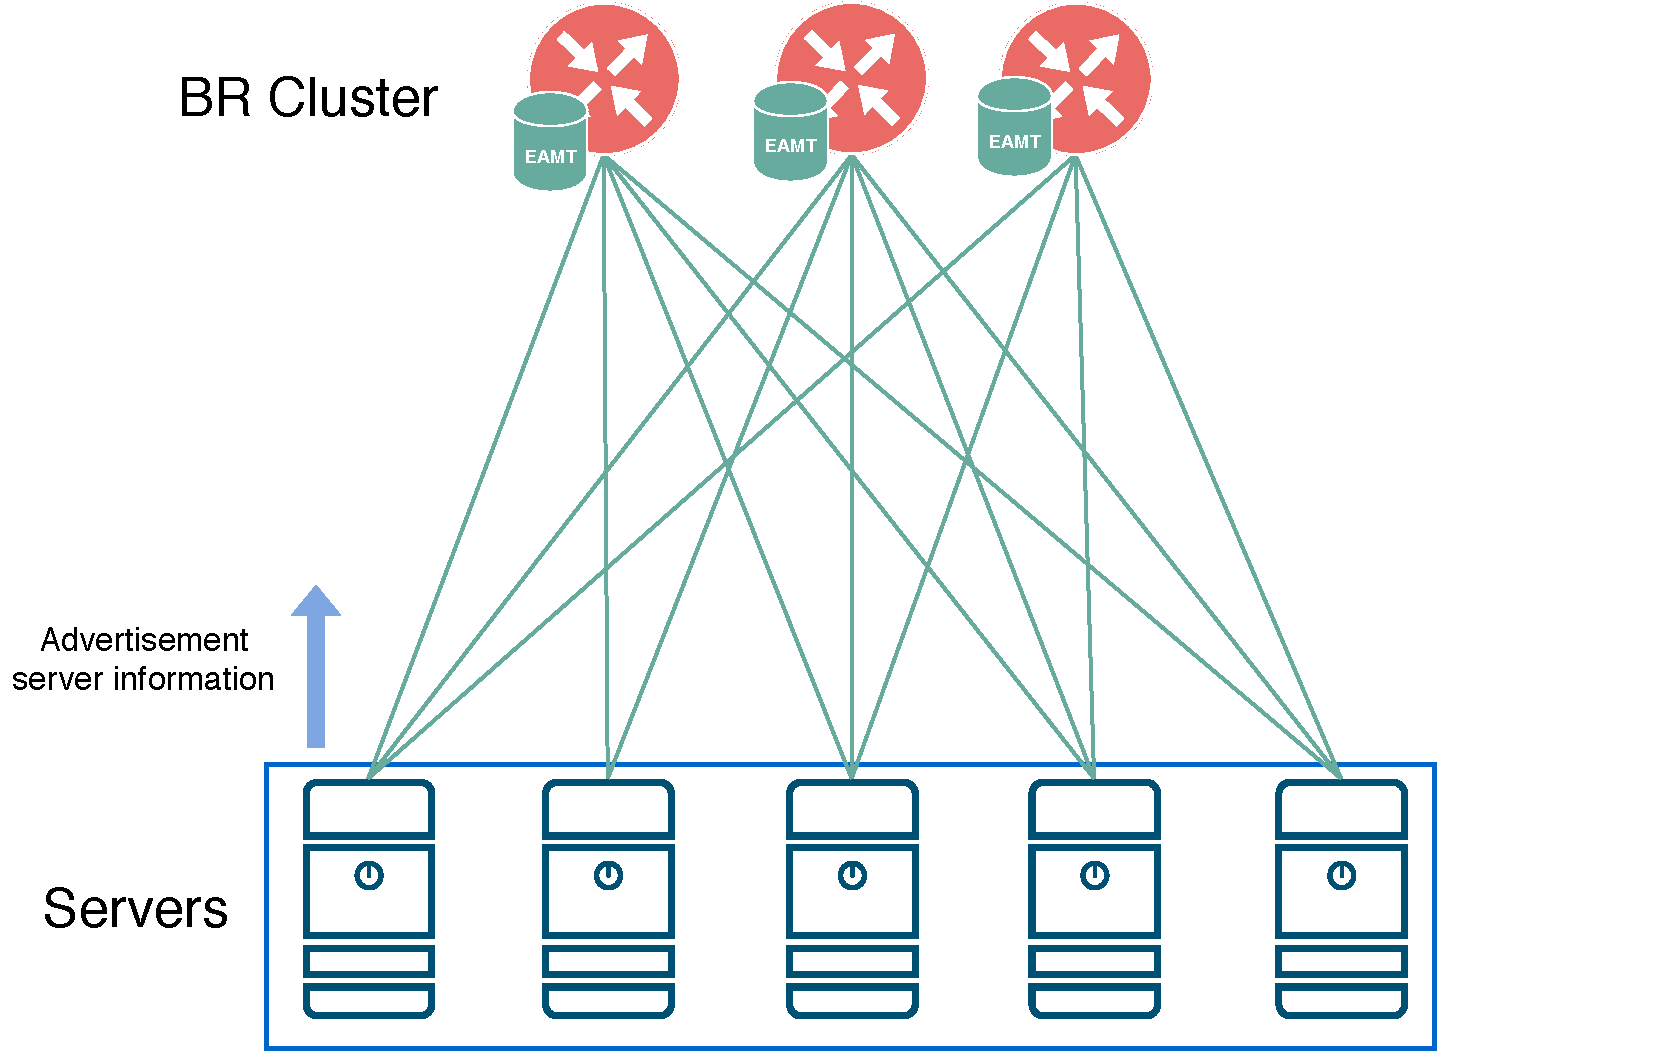
\includegraphics[width=12cm,pagebox=cropbox,clip]{img/approach_distributed_model.pdf}
    \end{center}
    \caption{分散管理型アプローチによるダイナミックEAMT}
    \label{fig:approach_distributed_model}
\end{figure}

\subsubsection{要件評価}

\begin{itemize}
    \item BR間のEAMTの一貫性 \\
    各BR間でEAMT一貫性を保証する機構は無いが,当該BRと疎通できないサーバーは障害時に自身のIPv4サービスアドレう宛のトラフィックを当該BRに経由させることが出来ないため,問題にならない.
    \item 変更追従性 \\
    サーバー自身のエージェントプロセスが直接BRに広告を行うため,実際の変更にリニアに対応出来る.
    \item スケーラビリティ \\
    EAMTの制御に必要とする通信コネクション数$C$は以下の通りになる.
    \begin{equation}
        C =  M \cdot N 
    \end{equation}
    サーバー群・各BR間でフルメッシュでのコネクションが必要なため,SIIT-DCネットワーク自体が小規模の場合のみ採用可能である.

    \item デプロイメントの容易さ \\
    各サーバー・BRにエージェントを導入する必要があるが,システム自体の機能は軽量である.
\end{itemize}

\section{アプローチの検討}

中央管理型アプローチが各BR間でのEAMT一貫性,スケーラビリティの二要素で優位であるが,コントローラーの役割が非常に大きくなり機能要件が高くなるため,変更追従性とデプロイメントの容易さの面での障壁が高いという問題も抱えている.一方で分散管理型アプローチはシンプルな構成であるためデプロイメントが比較的容易であり変更への追従がリニアであるが,各サーバーが通信コネクションを多量に貼らなくてはならない点でスケーラビリティに難がある.

本提案手法では両アプローチを総合した動的経路制御プロトコルであるiBGPを利用したハイブリッド型アプローチを提案する.第\ref{proposal}章において,本提案手法を中央管理型・分散型の両アプローチと比較する.


%%% Local Variables:
%%% mode: japanese-latex
%%% TeX-master: "../bthesis"
%%% End:
